\documentclass[aspectratio=169,compress]{beamer}
\usetheme[university=bs,faculty=standard]{fibeamer}
\usepackage[utf8]{inputenc}
\usepackage[
  main=english
]{babel}        %% typeset as follows:
%%
%%   \begin{otherlanguage}{italian}   ... \end{otherlanguage}
%%
%% These macros specify information about the presentation
\title{Typing Dynamic Languages with Set-Theoretic Types:\\
  The Case of Elixir}
\subtitle{\mbox{ }\vspace{6mm}
} %% title page.
\author{Giuseppe CASTAGNA
\hfill\parbox[t]{.2\textwidth}{
\footnotesize\it
Elisir di sì perfetta,\\[-1.5mm]
di sì rara qualità,\\[-1.5mm]
ne sapessi la ricetta,\\[-1.5mm]
conoscessi chi ti fa!
}\\\small
(joint work with Guillaume Duboc and José Valim)}
%% These additional packages are used within the document:
\usepackage[overlay,absolute,
%showboxes
]{textpos}
\usepackage{ragged2e}  % `\justifying` text
\usepackage{booktabs}  % Tables
\usepackage{tabularx}
\usepackage{tikz}      % Diagrams
\usetikzlibrary{calc, shapes, backgrounds}
\usepackage{amsmath, amssymb}
\usepackage{url}       % `\url`s
\usepackage{listings}  % Code listings
\usepackage{setup}
\usepackage{ulem}
\usepackage[cal=boondox,  % heavily sloped
            scr=esstix]   % slightly sloped
           {mathalpha}
\newtagform{purple}{\color{purple}(}{)}
%\frenchspacing

\newcommand{\struct}[1]{\textcolor{lightblue}{#1}}
% Beamer customization%%
\setbeamerfont{frametitle}{shape=\bf,size=\LARGE}
\addtobeamertemplate{frametitle}{\vspace*{-.4cm}}{\vspace*{0.2cm}}

\newenvironment<>{myblock}[1]{%
  \setbeamercolor{block title}{fg=cadmiumgreen,bg=white}%
  \setbeamercolor{block body}{fg=black,bg=white}%
  \setbeamerfont{block title}{size=\large,shape=\bf}
  \begin{block}#2{{#1}\vspace{-1.5mm}}}{\end{block}}

%%%% UNCOMMENT THE FOLLOWING LINE TO REMOVE SLIDE NUMBERS
%\setbeamertemplate{footline}{}

\begin{document}
  \frame[c]{\maketitle}

  %% \AtBeginSection[]{% Print an outline at the beginning of sections
  %%   \begin{frame}<beamer>
  %%     \frametitle{Outline for Section \thesection}
  %%     \tableofcontents[currentsection]
  %%   \end{frame}}

\section{Set-Theoretic Types and Dynamic Languages}
\begin{frame}
\frametitle{Outline} 
\tableofcontents
\end{frame}

\begin{frame}
\transdissolve<2->
\frametitle{Set-theoretic types}

We consider the following possibly recursive types:

{\Bl$$\T\ ::=\  \Bool\,\mid\,\Int\,\mid\,\pair\T\T\,\mid\,\T\To\T \,\mid\,{\color{darkgreen}\T\Or\T}\,\mid\,{\color{darkgreen}\T\!\And\!\T} \,\mid\, {\color{darkgreen} \neg\T}\,\mid\,{\color{darkred}\Any}\,\mid\,{\color{darkred}\Empty}\,\color<1>{white}\mid\,~\textcolor<2>{magenta}{\alpha} \color<2>{white}\,\mid\, \color<3>{magenta}{c} $$}

\pause\pause\pause\pause\pause
\bigskip

\textbf{Necessary to precisely capture the programming style used with dynamic languages:}
\begin{enumerate}
\item non-uniform structures/branching (union types, singletons)
\item overloading (intersection types)
\item pattern matching (negation types, ...)
\end{enumerate}


\textbf{\color<-6>{white}\color<7>{darkslateblue}Let us see each point more in detail}

\bigskip

\vfill

\small\color{gray} Note: henceforward I will sometimes use $\Bl\T_1\texttt{|}\T_2$ to denote $\Bl\T_1\Or\T_2$

\only<2>{\begin{textblock}{5}(0,0)
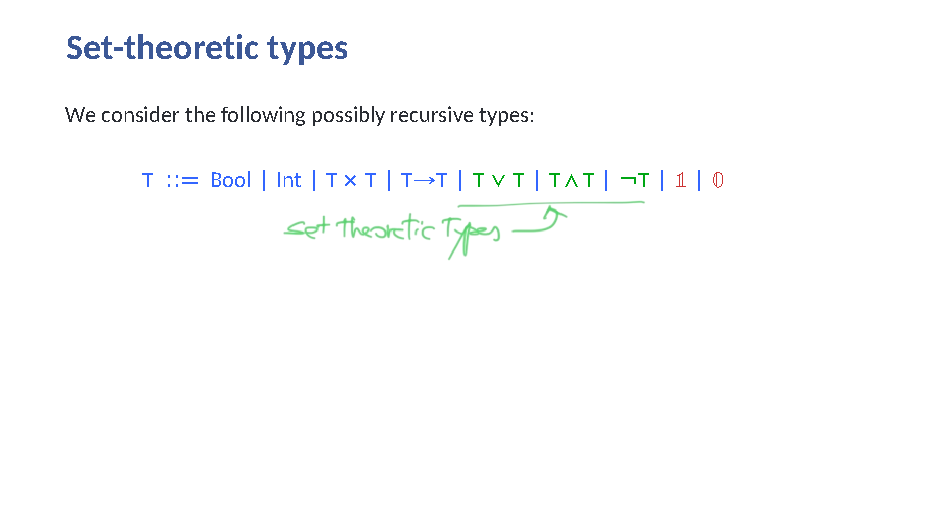
\includegraphics[scale=1]{images/slide-settheore.pdf}
\end{textblock}}
\only<3>{\begin{textblock}{5}(0,0)
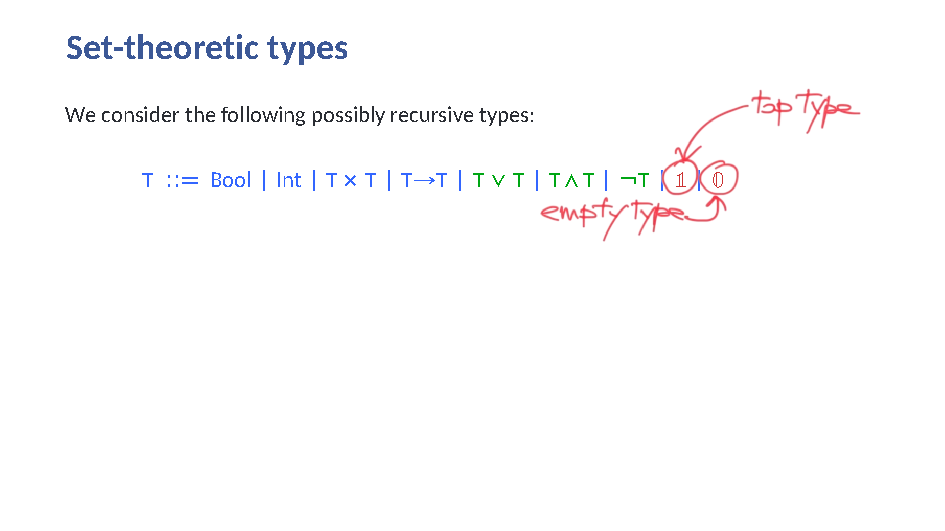
\includegraphics[scale=1]{images/slide-topbottom.pdf}
\end{textblock}}
\only<4>{\begin{textblock}{5}(0,0)
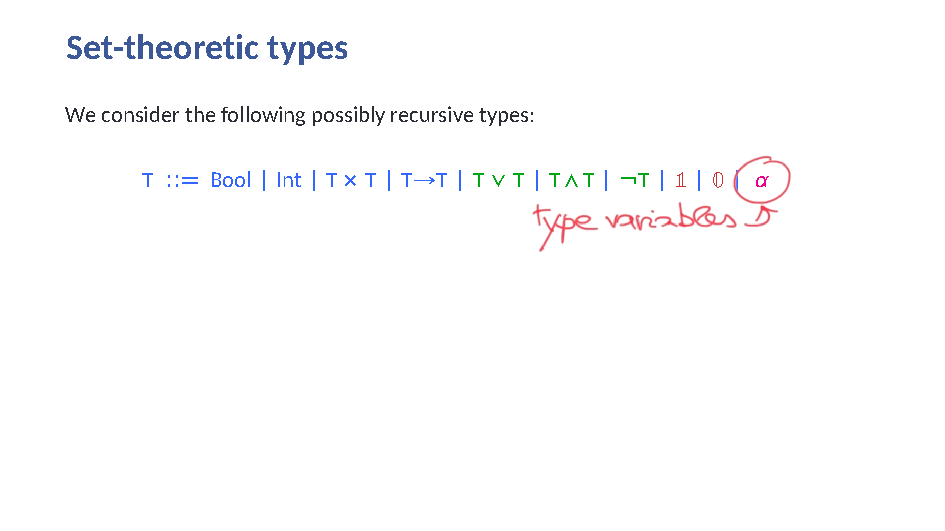
\includegraphics[scale=1]{images/slide-variables.pdf}
\end{textblock}}
\only<5>{\begin{textblock}{5}(0,0)
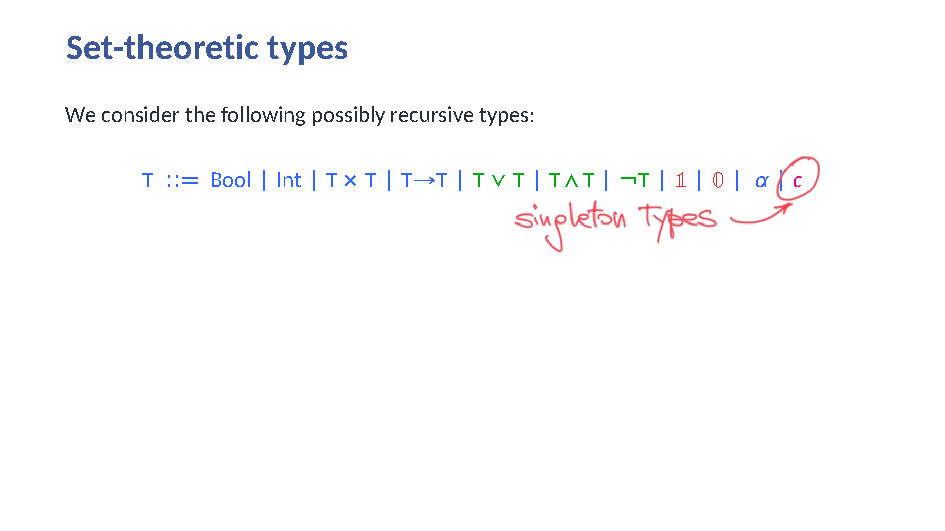
\includegraphics[scale=1]{images/slide-singleton.pdf}
\end{textblock}}
\end{frame}

\subsection{Branching, overloading, and pattern matching}

\begin{frame}[fragile]\transdissolve
\frametitle{1. Branching and discriminated unions}\vspace{-4mm}
\small
\begin{minted}{TypeScript}
type Status = "pending" | "success" | "error";
type Result = string | number | boolean;
function processStatus(input: Status): Result {
  switch (input) {
    case "pending":
      return "Processing...";       // returns string
    case "success":
      return 200;                   // returns number
    case "error":
      return false;                 // returns boolean
    default:
      return "Unknown status";      // returns string
  }
}
\end{minted}
\pause


% Discriminated unions are a common pattern in dynamic languages to handle different types of data structures that share some common properties.
\begin{minted}{TypeScript}
type PaymentMethod = 
  | { type: "credit_card"; cardNumber: string; cvv: string }
  | { type: "paypal"; email: string }
  | { type: "bank_transfer"; accountNumber: string; routingNumber: string };
\end{minted}
\end{frame}



\begin{frame}[fragile]\transdissolve
  \frametitle{2. Overloading: basic use}
 \structure{\bf Aka \emph{ad hoc} polymorphism: functions that execute different code on arguments of different types}

\smallskip

\begin{minted}{TypeScript}
function double (x) {
    return (typeof(x) === "number") ? 2*x : x.concat(x);
}
\end{minted}
\textcolor<4>{red}{If applied to an integer returns an integer, if applied to a string returns a string}
  \pause
\begin{exampleblock}{Use set-theoretic types}
  \begin{itemize}
    \pause
     \item Naive solution: union types
       \centerline{\pb{(number|string)$\to$(number|string)}}
       \pause\pause
     \item Better solution: intersection types
       \centerline{\pb{\color<6>{darkred}(number$\to$number) \& (string$\to$string)}}
  \end{itemize}
\end{exampleblock}
\end{frame}


\begin{frame}[fragile]
\frametitle{2. Overloading: advanced use}
\begin{minted}{TypeScript}
function toBoolean(x) {
    if (x === 0 || x === "" || x == null || Number.isNaN(x)) return false;
    return true;
}

function logicalOr(x, y) {
    if (toBoolean(x)) return x; return y;
}
\end{minted}
\pause

\bigskip

\begin{exampleblock}{Fine grained typing to capture the code semantics}
\color{typeBlue}
\tt
type Falsy = 0 | "" | null | undefined | NaN;

type Truthy = $\neg$Falsy;

toBoolean : (Truthy $\to$ true)  $\wedge$ (Falsy $\to$ false)

logicalOR : \ (($\alpha{\wedge}$Truthy$\,\times\,\Any$)$ \to \alpha$)  $\wedge$ ((Falsy$\times \beta$)$\,\to \beta$)

\end{exampleblock}
\end{frame}




\begin{frame}[fragile]
\frametitle{3. Precise typing of pattern matching (I)}
Consider the following pattern matching expression
 
\hspace*{5mm}{\Bl$\texttt{ match }  e  \texttt{ with } p_1 \texttt{ -> } e_1 \texttt{ | } p_2\texttt{ -> } e_2$}

where patterns are defined as follows:
\centerline{$\Bl p ::= x \ \mid\  \patpair{p}{p} \ \mid\ \pator{p}{p}\ \mid\ \patand{p}{p} $}
\pause
If we interpret types as set of values
\centerline{$\Bl
t = \{ v\mid v\text{ is a value of type }t\}$}
\pause
then \textbf{\color{darkslateblue}the set of all values that match a pattern is a type}
\centerline{\color{magenta}
$\accept{p} = \{ v\mid v\text{ is a value that matches }p\}
$}
\vspace{-9mm}
{\color{lightgray}
\begin{eqnarray*}
\accept x  & = & \Any\\[-1.5mm]
\accept{\patpair{p_1}{p_2}}  & = & \pair{\accept{p_1}}{\accept{p_2}}\\[-1.5mm]
\accept{\pator{p_1}{p_2}} & = & {\accept{p_1}}\Or{\accept{p_2}}\\[-1.5mm]
\accept{\patand{p_1}{p_2}} & = &{\accept{p_1}}\And{\accept{p_2}}
\end{eqnarray*}
}
\pause\pause\vspace{-9mm}

\textbf{\color{darkslateblue}Let us see how to type pattern matching.}
\only<4>{\begin{textblock}{5}(0,0)
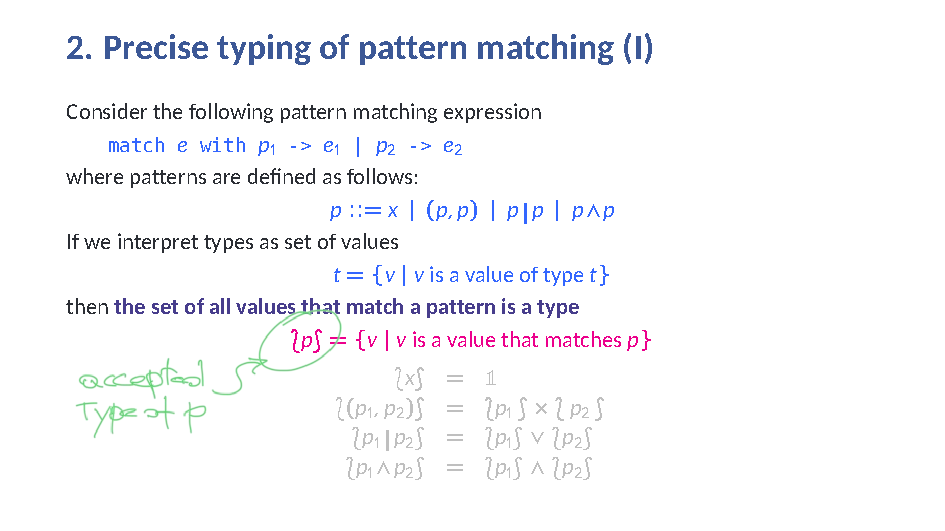
\includegraphics[scale=1]{images/slide-accepted.pdf}
\end{textblock}}
\end{frame}



\begin{frame}
\frametitle{3. Precise typing of pattern matching (II)}\transdissolve<10>

\textbf{Boolean type connectives are needed to type pattern matching:}

\pause
\smallskip

    \hspace*{5mm}{\Bl$\texttt{ match }  e  \texttt{ with } p_1 \texttt{ -> } e_1 \texttt{ | } p_2\texttt{ -> } e_2$}\pause

   \smallskip

Suppose that $\Bl e:\T$ and let us write $\Bl\T_1\setminus\T_2$ for $\Bl\T_1\!{\And}\!\neg{\T_2}$\\[-2mm]

\pause

  - To infer the type $\Bl\T_1$ of $\Bl e_1$ we need {\color{blue}$\T{\color<8->{magenta}\mypmb<8->{\And}}\accept{p_1}$};

\pause

  - To infer the type $\Bl\T_2$ of $\Bl e_2$ we need {\color{blue}$(\T{\color<8->{magenta}\,\mypmb<8->{\backslash}}\accept{p_1}){\color<8->{magenta}\mypmb<8->{\And}}\accept{p_2}$;}

\pause

  - The type of the match expression is {\color{blue}$\T_1{\color<8->{magenta}\mypmb<8->{\Or}} T_2$ }.

\pause

  - Pattern matching is exhaustive if $\color{blue}\T\leq\accept{p_1}{\color<8->{magenta}\mypmb<8->{\Or}}\accept{p_2}$;


\pause\pause
\textbf{Formally:}
\vspace{-2mm}
\begin{mathpar}\Bl
\infer[{[Match]}]
{\Gamma\vdash e:\T\and\Gamma, \T\!\!\And\!\!\accept{p_1\!}/p_1\vdash e_1:\T_1\and \Gamma, \T\setminus\accept{p_1\!}/p_2\vdash e_2:\T_2}
{\Gamma\vdash \texttt{match } e \texttt{ with }p_1 \texttt{->} e_1 \texttt{ | }p_1 \texttt{->} e_2 : \T_1\Or\T_2 }\mbox{\small($\T\leq\accept{p_1\!}\Or\accept{\!p_2\!}$)}
\end{mathpar}
\vspace{-4mm}

\small\color{gray}
where $\Bl \T/p$ is the type for the capture variables in $\Bl p$ when it is matched against values in $\Bl \T$.

\only<10>{\begin{textblock}{5}(0,0)
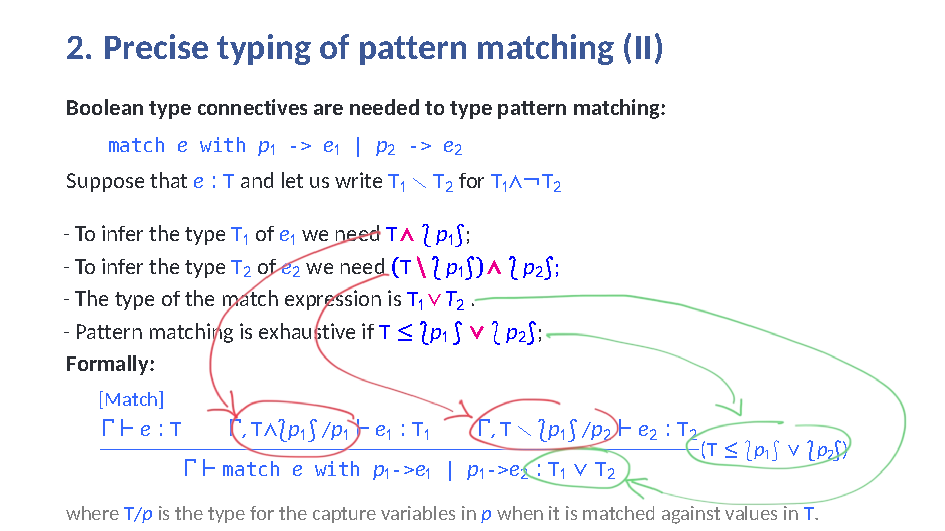
\includegraphics[scale=1]{images/slide-caseexp.pdf}
\end{textblock}}
\end{frame}

\subsection{Semantic subtyping}
\begin{frame}
\frametitle{Semantic subtyping}

Many dynamic languages support union and intersection types: TypeScript, Flow, Hack, Python, Julia, and Ceylon. Negation types are less common: TypeScript (with the `Exclude` utility type) and Scala (with `Not` type constraints).

\pause\bigskip

\textbf{What differentiates our approach is the use of \emph{semantic subtyping} to define\\  the subtyping relation for union, intersection, and negation types.}

\bigskip

\begin{enumerate}
  \item<3-> Define a set-theoretic interpretation of types as sets of values
  \item<4-> Define union, intersection, and negation types as set-theoretic operations
  \item<5-> Define the subtyping relation as a set-theoretic inclusion relation
  \item<6-> Deduce from this how to decide the subtyping relation and compute type operators
  \end{enumerate}

\end{frame}

\begin{frame}\transdissolve
\frametitle{Semantic subtyping: in practice}
\pause
\begin{enumerate}
\item<2-> $\begin{array}[t]{lcl}
  \sem{Int} & = & \{ n \mid n \text{ is an integer} \}\\[-1mm]
  \sem{Bool} & = & \{ \texttt{true}, \texttt{false} \}\\[-1mm]
  \sem{\T_1\to\T_2} & = & \{ f \mid v\in\sem{\T_1}\implies f(v)\in\sem{\T_2} \}\\[-2mm]
  &\vdots
\end{array}$
\item<3-> ~~$\sem{\T_1\Or\T_2} = \sem{\T_1}\cup\sem{\T_2}, \quad
\sem{\T_1\And\T_2} = \sem{\T_1}\cap\sem{\T_2}, \quad
\sem{\neg\T} = \{ v \mid v\notin\sem{\T} \}$\\[4mm]
\item<4-> ~~$\T_1\leq\T_2 ~~\stackrel{def}{\Longleftrightarrow}~~ \sem{\T_1}\subseteq\sem{\T_2} ~~\Longleftrightarrow ~~ \sem{\T_1}\cap\sem{\neg\T_2}=\varnothing ~~ \Longleftrightarrow ~~ \T_1\And\neg\T_2\leq\Empty$\\
\item<5-> $\color{cadmiumgreen}
\begin{array}{l}
\displaystyle
\syncap_{i \in I} t_i \syntimes s_i \leq
  \syncup_{i \in J} t_i \syntimes s_i ~~\iff~~
\forall J' \subset J.~
\left(
\syncap_{i \in I} t_i \leq \syncup_{i \in J'} t_i
\right)
\mbox{or}
\left(
\syncap_{i \in I} s_i \leq \syncup_{i \in J \backslash J'} s_i
\right)
\end{array}
$
\end{enumerate}
\pause\pause\pause\pause
\begin{block}{Paying the price}
  \begin{itemize}\color{newgreen}
    \item[\textcolor{newgreen}{\ding{52}}] Unions, intersections, and negations are \emph{\sl really} set-theoretic\color{red}
    \item[\textcolor{red}{\ding{56}}] Simply extending syntactic subtyping is not an option
  \end{itemize}
\end{block}

\end{frame}



\begin{frame}
\frametitle{Theoretical foundations}
\begin{itemize}
\item<1-> Semantic Subtyping for Set-Theoretic Types (JACM 2008)    
\item<2-> Polymorphic Types and Subtyping (ICFP 2011)
\item<3-> Typing of Polymorphic Functions and Local Type Inference (POPL 2014, POPL 2015)
\item<4-> Gradual Typing (POPL 2019)
\item<5-> Monomorphic Type Reconstruction (POPL 2022)
\item<6-> Uniform Typing for Records and Dictionaries (ICFP 2023)
\item<7-> Polymorphic Type Reconstruction and Occurrence Typing (POPL 2024)
\item<8-> Row Polymorphism (OOPSLA 2025)
\item<9-> First-class Modules (in progress)
\end{itemize}
\end{frame}

\begin{frame}
\frametitle{Set-theoretic types: state of the art}
\transdissolve<2>
\includegraphics<1>[width=.7\textwidth]{images/POPL24 1.png}
\includegraphics<2->[width=.7\textwidth]{images/POPL24.png}
\only<3>{
\begin{textblock}{12}(2.9,7.8)\small\color{purple}
    $\forall(\alpha{\leq}\texttt{Truthy})\forall(\beta)\,.\, (\alpha,\texttt{Any}\to\alpha)\wedge(\texttt{Falsy},\beta\to\beta)$
\end{textblock}
\begin{textblock}{12}(2.9,12.3)\small\color{purple}
    $\forall(\alpha)\forall(\beta)\forall(\gamma)\,.\, ((\alpha\to\beta)\to((\alpha\to\beta)\wedge\gamma))\to((\alpha\to\beta)\wedge\gamma)$
\end{textblock}}
\end{frame}




\section{Elixir basic typing}

\begin{frame}
\frametitle{Outline} 
\tableofcontents[currentsection]
\end{frame}

\begin{frame}
\frametitle{Putting the theory to work: Elixir}
\begin{itemize}
\item<1-> Elixir is a dynamic language with a strong emphasis on metaprogramming
\item<2-> It is a functional language with a syntax similar to Ruby
\item<3-> It is built on top of the Erlang VM, which provides a powerful runtime system for distributed and fault-tolerant applications
\item<4-> It has a rich ecosystem of libraries and frameworks and a strong community of nearly 100K developers (with the highest median salaries cf.\  2024 Stack Overflow survey)
\item<5-> It is used in production by companies like Discord, Pinterest, PepsiCo, ...
\item<6-> Since 2021 we have been collaborating with José Valim, the creator of Elixir, and the Dashbit team to develop a type system for Elixir.
\item<7-> The static type system is based on the set-theoretic types we have developed in the past years and being gradually integrated into the Elixir compiler since version 1.17 (the current version is 1.19).
\end{itemize}
\end{frame}


\subsection{Simple function types}


\begin{frame}[fragile]
\frametitle{Static Typing 101}
\begin{block}{A function that always errors}
\begin{minted}[escapeinside=!!]{elixir}
def negate(x) when is_integer(x), do: not x
\end{minted}
\end{block}\pause
\begin{block}{Type error message}
\begin{minted}[escapeinside=!!]{elixir}
Type error:
  |  def negate(x) when is_integer(x), do: not x
                                           ^^^^^
        the operator not expects boolean() as arguments,
        but the argument is integer()
\end{minted}
\end{block}
\end{frame}



% \defverbatim[colored]{\intToInt}{
% \begin{minted}{elixir}
% !\spec! !\po!integer() !\arr! integer()!\pc!
% \end{minted}
% }
\defverbatim[colored]{\intToInt}{
\begin{coloredverbatim}
$ (integer() -> integer())
\end{coloredverbatim}
}
\defverbatim[colored]{\negateInt}{
\begin{minted}{elixir}
def negate(x) when is_integer(x), do: -x
\end{minted}
}

\begin{frame}[fragile]
\frametitle{Types as contracts between functions.}
\pause
\begin{block}{Function A: Negate}
\visible<3->{%
\intToInt
}
\vspace{-2mm}
\visible<2->{%
\negateInt
}
\vspace{-1.8mm}
\end{block}
\pause\pause
\begin{block}{Function B: Subtract}
\vspace{-1mm}
\begin{coloredverbatim}
$ (integer(), integer() -> integer())
\end{coloredverbatim}
\vspace{-2mm}
\begin{minted}[escapeinside=!!]{elixir}
def subtract(a, b) when is_integer(a) and is_integer(b) do
    a + negate(b)
end
\end{minted}
\end{block}
\pause
\begin{block}{Question}
\begin{itemize}
    \item What if we modify the implementation of \code{negate}?
\end{itemize}
\end{block}
% \begin{block}{Answer}
% If the implementation of \code{negate} changes and violates the type contract, it could lead to unexpected behavior or errors in the \code{subtract} function. Ensuring that the contract is maintained helps guarantee the correctness of our code.
% \end{block}
\end{frame}

\defverbatim[colored]{\intBool}{
\begin{coloredverbatim}
$ (integer() \oor boolean()) -> (integer() \oor boolean())
\end{coloredverbatim}
}
\defverbatim[colored]{\negateBool}{
\begin{minted}{elixir}
def negate(x) when is_boolean(x), do: not x
\end{minted}
}



\subsection{Unions, intersections, negations}

\begin{frame}[fragile]{Union types: correct, but not precise enough.}
\vspace{-2mm}
\begin{block}{Adding a clause for booleans}
\visible<2->{%
\intBool
}
\vspace{-2.1mm}
\visible<1->{%
\negateInt
\vspace{-2.1mm}
\negateBool
}
\vspace{-2.2mm}
\end{block}
\pause\pause

\vspace{-4mm}

\begin{block}{\vspace{-5mm}}
\vspace{-0.2mm}
\begin{coloredverbatim}
$ (integer(), integer() -> integer())
\end{coloredverbatim}
\vspace{-2.1mm}
\begin{minted}[escapeinside=!!]{elixir}
def subtract(a, b) when is_integer(a) and is_integer(b) do
    a + negate(b)
end
\end{minted}
\end{block}
\pause
\begin{block}{Type error in subtract}
\begin{minted}[fontsize=\footnotesize]{elixir}
Type error:
  | def subtract(a, b) when is_integer(a) and is_integer(b) do
  |   a + negate(b)
        ^ the operator + expects integer(), integer() as arguments,
          but the second argument can be integer() or boolean()
\end{minted}
\end{block}
\end{frame}
% todo: add notes with pdfpc
% \begin{block}{Explanation}
% The `+` operator expects two integer arguments, but the second argument can now be an integer \emph{or} a boolean due to the changes in the `negate` function. 
% \end{block}
\defverbatim[colored]{\intersection}{
\begin{coloredverbatim}
$ (integer()->integer()) \oand (boolean()->boolean())
\end{coloredverbatim}
}
\defverbatim[colored]{\intersectionHalf}{
\begin{coloredverbatim}
$ (integer()->integer()) \oand
\end{coloredverbatim}
}
\defverbatim[colored]{\negateIntBool}{
\begin{minted}[escapeinside=!!]{elixir}
def negate(x) when is_integer(x), do: -x
def negate(x) when is_boolean(x), do: not x
\end{minted}
}

\defverbatim[colored]{\intersection}{
\begin{coloredverbatim}
$ (integer()->integer()) \oand (boolean()->boolean())
\end{coloredverbatim}
}
\defverbatim[colored]{\intersectionHalf}{
\begin{coloredverbatim}
$ (integer()->integer()) \oand
\end{coloredverbatim}
}
\defverbatim[colored]{\negateIntBool}{
\begin{minted}[escapeinside=!!]{elixir}
def negate(x) when is_integer(x), do: -x
def negate(x) when is_boolean(x), do: not x
\end{minted}
}


\begin{frame}[fragile]
\frametitle{Type intersections for functions.}
\begin{block}{A more precise annotation}
\vspace{-4.9mm}
\begin{overlayarea}{\textwidth}{.8cm}
% \only<2>{\intersectionHalf}
\only<2->{\intersection}    
\end{overlayarea}
\vspace{.4mm}
% \hfill
% \vspace{1mm}
\negateIntBool
\vspace{-0.7mm}
\end{block}
\pause\pause
\begin{block}{The function \texttt{subtract} type checks}
\vspace{-2mm}
\begin{coloredverbatim}
$ (integer(), integer() -> integer())
\end{coloredverbatim}
\vspace{-2.1mm}
\begin{minted}[escapeinside=!!]{elixir}
def subtract(a, b) when is_integer(a) and is_integer(b) do
    a + negate(b)
end
\end{minted}
\end{block}
\end{frame}

\defverbatim[colored]{\lognegType}{
\begin{coloredverbatim}
$ (false \oor nil -> true) \oand (\onot (false \oor nil) -> false)
\end{coloredverbatim}
}
\defverbatim[colored]{\lognegSingle}{
\begin{coloredverbatim}
$ (false \oor nil -> true) \oand
\end{coloredverbatim}
}

\begin{frame}[fragile]
\frametitle{Singleton and Negation Types}
\begin{block}{Logical negation}%
\vspace{-9mm}
\begin{overlayarea}{\textwidth}{0.5mm}%
    \only<2>{\lognegSingle}
\only<3>{\lognegType}
\end{overlayarea}%
\hfill \vspace{1mm}
\begin{minted}[escapeinside=||]{elixir}
def logical_neg(x) when x == false or x == nil, do: true
def logical_neg(x), do: false
\end{minted}
\end{block}
\pause
\begin{block}{Types}
\begin{itemize}
    \item Singleton types are types containing exactly one value
    \visible<3->{\item Negation types contain any value that is \emph{not} in the 
    negated type.}
\end{itemize}
\end{block}

\end{frame}

\defverbatim[colored]{\mapSip}{
\begin{coloredverbatim}
$ ([a], (a -> b)) -> [b] \owhen a: term(), b: term()
\end{coloredverbatim}
}
\defverbatim[colored]{\mapSigMinted}{
\begin{minted}{elixir}
!\spec! ([a], (a -> b)) -> [b] !\when! a: term(), b: term()
\end{minted}
}
\defverbatim[colored]{\map}{
\begin{minted}[escapeinside=!!]{elixir}
def map([h | t], fun), do: [fun.(h) | map(t, fun)]
def map([], _fun), do: []
\end{minted}
}


\subsection{Polymorphism}
\begin{frame}[fragile]
\frametitle{Polymorphism with Local Type Inference}

\begin{block}{Expressions and functions can have types containing type variables}
\vspace{-7.2mm}
\begin{overlayarea}{\textwidth}{2mm}
\only<2->{\mapSip}
% \only<2->{\mapSigMinted} 
\end{overlayarea} 
\hfill \vspace{1.4mm}
\visible<1->{\map}
\vspace{-1.5mm}
\end{block}
\pause
\begin{block}{Type Variables}
    \begin{itemize}
        \item Quantified using a postfix \texttt{\color{typeBrique}when} with upper bounds
        % \item First-order polymorphism only
    \end{itemize}
\end{block}
\pause
\begin{block}{System deduces type variable instantiation}
\begin{minted}{elixir}
map([{0, true}], fn {x, y} when is_integer(x) -> x end)
# type [integer()]
\end{minted}
\end{block}
\end{frame}

\defverbatim[colored]{\logorFinal}{
\begin{coloredverbatim}
$ ((false \oor nil, a) -> a) when a: term()
$ (a, term() -> a) when a: \onot(false or nil)
\end{coloredverbatim}
}
\defverbatim[colored]{\logorFirst}{
\begin{coloredverbatim}
$ ((false \oor nil, a) -> a) \oand 

\end{coloredverbatim}
}
\defverbatim[colored]{\logorSecond}{
\begin{coloredverbatim}
$ ((false \oor nil, a) -> a) \oand 
  ((b, term()) -> b) \owhen a: term(), b: \onot(false \oor nil)
\end{coloredverbatim}
}


\begin{frame}[fragile]{Intersection and polymorphism}\transdissolve<4->

\begin{block}{Logical OR}%
\vspace{-7mm}
\begin{overlayarea}{\textwidth}{2mm}
    \only<2>{\logorFirst}
    \only<3->{\logorSecond}
    % \only<4>{\logorFinal}
\end{overlayarea}%
\hfill \break 
\begin{minted}[escapeinside=!!]{elixir}
def logical_or(x, y) when x == false or x == nil, do: y
def logical_or(x, _), do: x
\end{minted}
\end{block}
\pause\pause\pause\pause
\textbf{\color{darkslateblue}Bounded Polymorphism:}
\[\color{typeBrique}\forall (s{\leq}\alpha{\leq} u).t \quad\stackrel{def}{=}\quad (\forall \alpha).t[\alpha:=(s{\vee}(\alpha{\wedge} u))]\]
\only<4>{\begin{textblock}{5}(0,0)
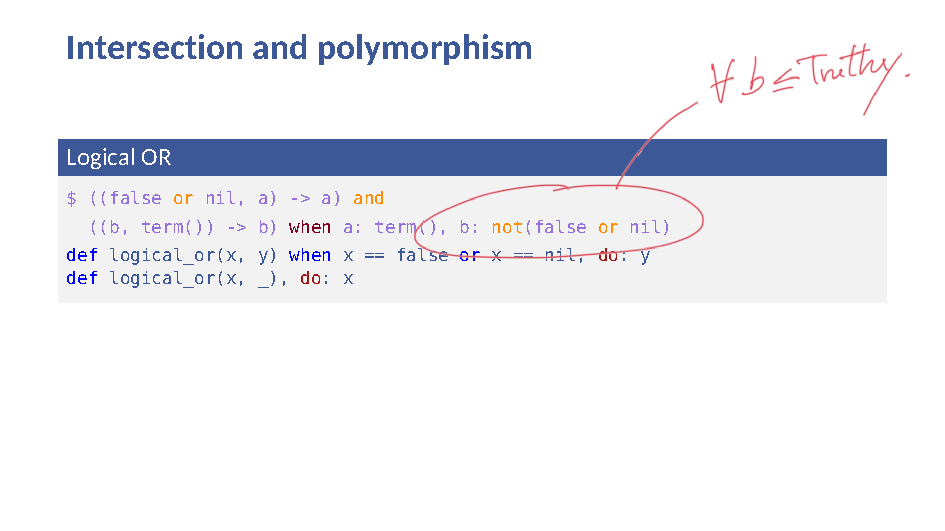
\includegraphics[scale=1]{images/slide-bounded_q.pdf}
\end{textblock}}
\end{frame}





\section{Guard Analysis}
\begin{frame}
\frametitle{Outline} 
\tableofcontents[currentsection]
\end{frame}


\subsection{Case expressions: redundancy, exhaustiveness, and narrowing}

\begin{frame}[fragile]
\frametitle{Pattern Matching: Case expressions}
\begin{block}{Using a case expression}
\begin{minted}[escapeinside=!!]{elixir}
def negate(x), do: (case x do
  x when is_integer(x) -> -x
  x when is_boolean(x) -> not x
end)
\end{minted}
\end{block}

\begin{block}{Using multiple function clauses}
\begin{minted}[escapeinside=!!]{elixir}
def negate(x) when is_integer(x), do: -x
def negate(x) when is_boolean(x), do: not x
\end{minted}
\end{block}

\textbf{\color{darkslateblue}Both are equivalent, but the second is preferred in Elixir.}
\end{frame}

\defverbatim[colored]{\result}{
%\vspace{-1.5mm}
\begin{minted}[escapeinside=||,fontsize=\small]{elixir}
|\spec| |\ty| result() = 
    %{output: :ok, socket: socket()} or
    %{output: :error, message: :timeout or {:delay, integer()}}
\end{minted}
\vspace{-1.5mm}
}

\begin{frame}[fragile]
\frametitle{Exhaustiveness and redundancy checking}
\vspace{-7mm}
\begin{block}{\vspace{-5mm}}
\result
\end{block}
\pause

\begin{block}{Exhaustiveness checking: handling all cases}
\begin{minted}[escapeinside=||,fontsize=\small]{elixir}
|\spec| result() -> string()
def handle(r) when r.output == :ok, do: "Msg received"
def handle(r) when r.message == :timeout, do: "Timeout"
\end{minted}
\pause
\vspace{-1.8mm}
\begin{minted}[fontsize=\small]{elixir}
#=> Type Warning: non-exhaustive pattern matching
\end{minted}
\end{block}
\pause

\defverbatim[colored]{\unusedBranch}{
\begin{minted}[fontsize=\small]{elixir}
#=> Type Warning: unused branch
\end{minted}
}

\begin{block}{Redundancy checking: detecting unused clauses}
\begin{minted}[escapeinside=||,fontsize=\small]{elixir}
|\spec| result() -> string()
def handle(r) when r.output == :ok, do: "Msg received"
def handle(r) when r.output == :error, do: "Error raised"
def handle(%{socket: _}), do: "Socket found"
\end{minted}
\pause%
\vspace{-1.6mm}\unusedBranch\vspace{-1.7mm}
\end{block}
\end{frame}

% add a fourth branch for overlapping, by matching 
% on :socket

% remove? no time
\begin{frame}[fragile]
\transdissolve
\frametitle{Narrowing: inferring more precise types}

\vspace{-11mm}%was \vspace{-4mm}
\begin{block}{\vspace{-5mm}}
\result
\end{block}\pause
\begin{block}{Automatically infer a return type}
\begin{minted}[escapeinside=||,fontsize=\footnotesize]{elixir}
|\spec| result() -> _
def handle(r) when r.output == :ok, do: {:accepted, r.socket}
def handle(r) when is_atom(r.message), do: r.message
def handle(r), do: {:retry, elem(r.message, 1)}
\end{minted}
\pause\vspace{-1.7mm}
\begin{minted}[fontsize=\footnotesize]{elixir}
#=> Return type: {:accept, socket()} or :timeout or {:retry, integer()}
\end{minted}
\vspace{-1.2mm}
\end{block}
\pause\pause\pause\pause
\begin{block}{Inferring a more precise type}
\begin{minted}[fontsize=\footnotesize,escapeinside=||]{elixir}
|\spec| (%{output: :ok, socket: socket()} -> {:accept,socket()}) and
  (%{output: :error, message: :timeout} -> :timeout) and
  (%{output: :error, message: {:delay,integer()}} -> {:retry,integer()})
\end{minted}
\end{block}
\only<4>{\begin{textblock}{5}(0,0)
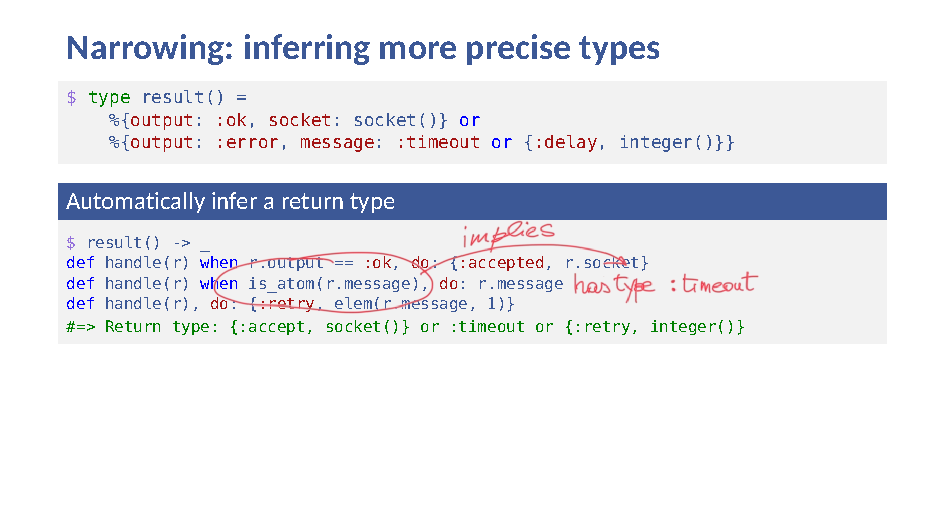
\includegraphics[scale=1]{images/slide-narrow1.pdf}
\end{textblock}}

\only<5>{\begin{textblock}{5}(0,0)
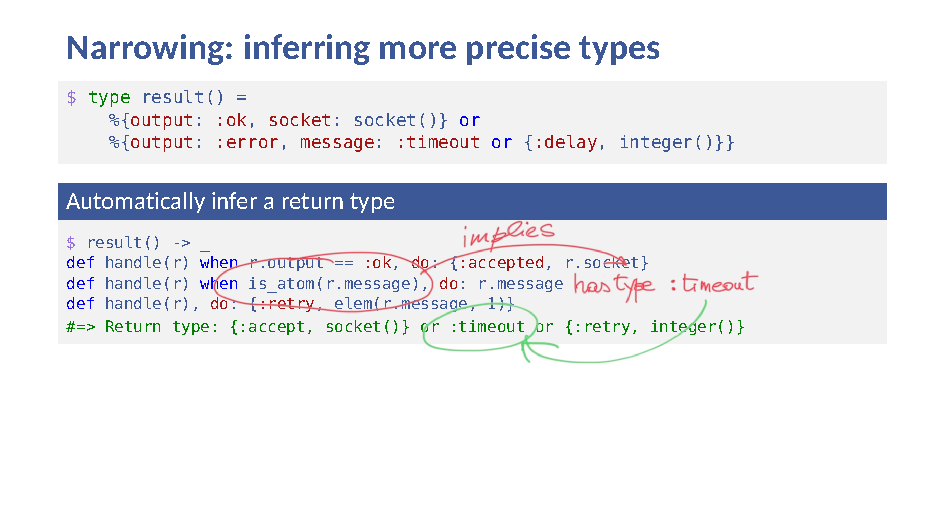
\includegraphics[scale=1]{images/slide-narrow2.pdf}
\end{textblock}}
\only<6>{\begin{textblock}{5}(0,0)
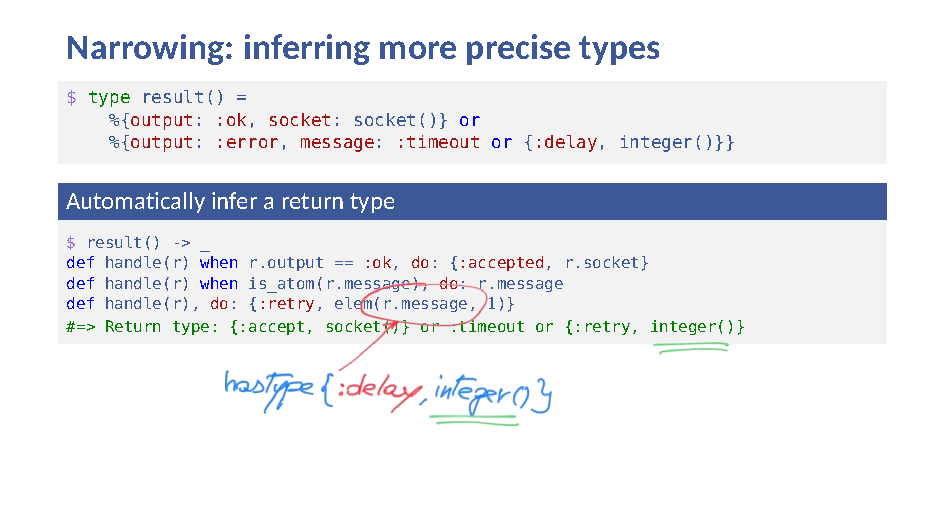
\includegraphics[scale=1]{images/slide-narrow3.pdf}
\end{textblock}}

\only<8>{\begin{textblock}{5}(0,0)
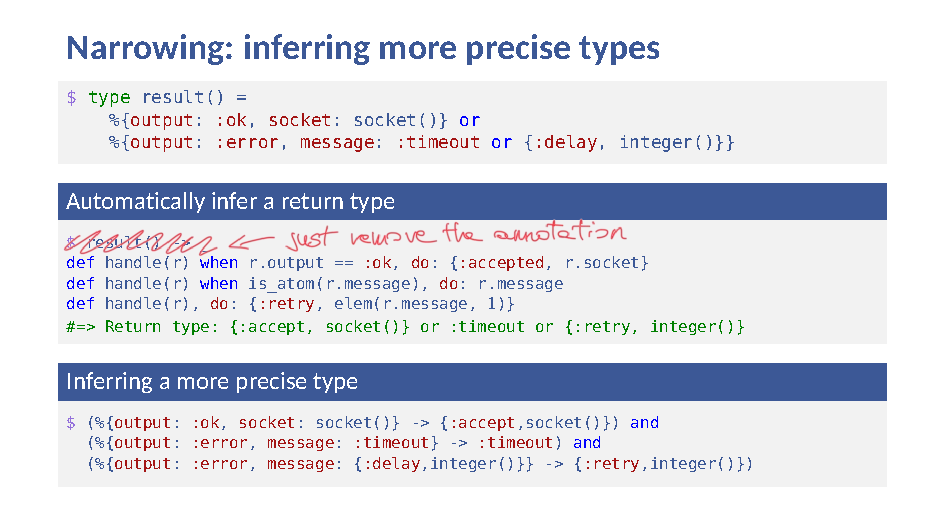
\includegraphics[scale=1]{images/slideNarrowing.pdf}
\end{textblock}}
\end{frame}



\renewcommand{\code}[1]{\mintinline{elixir}{#1}}
\subsection{A Pinch of Formalization}

\begin{frame}[fragile]
\frametitle{A Pinch of Formalization}\transdissolve
\color{darkslateblue}
\begin{minipage}{\textwidth}
\color<2->{gray}
  \begin{figure}
  \centering
  $\alpha$ type variables, $c$ constants, $x$ variables
  \begin{grammarfig}
    \text{Base types}  & b &\bnfeq& \intTop \bnfor \atomTop \bnfor \texttt{function} \bnfor \texttt{tuple} \\[1mm]
    \text{Types}       & t,s &\bnfeq& b \bnfor c  \bnfor \alpha \bnfor \fun{\ov{t}}{t}
    \bnfor  \tuple{\,\ov{t}\,} \color<2->{magenta}\bnfor t \lor t  \bnfor t\land t \bnfor \neg t\\[2mm]
    \text{Expressions} & e, f &\bnfeq& c\bnfor x\bnfor  \textcolor<2->{typeBlue}{\lam{\ov{x}}{e}}
    \bnfor\app{f}{\ov{e}}\bnfor\tuple{\,\ov{e}\,} \bnfor \elem{e}{e} \\[1.5mm]
    &&\bnfor& \tlet{x}{t}{e}{e}
    \bnfor \color<2->{typeBlue} \caseExpr{} \\[2mm]
\color<3>{newgreen}    \text{Patterns}
\color<3>{newgreen}    &p &\bnfeq& \color<3>{newgreen}x \bnfor c \bnfor \tuple{\,\ov{p}\,} \\[1mm]
\color<3>{newgreen}    \text{Guards}
\color<3>{newgreen}    &g &\bnfeq&\color<3>{newgreen} \gand{g}{g} \bnfor \gor{g}{g} \bnfor \gnot{g} \bnfor \isInt{d}  \\
\color<3>{newgreen}    &&\bnfor&\color<3>{newgreen} \isAtom{d} \bnfor \isTuple{d} \bnfor \isFunction{d}{d}  \\
\color<3>{newgreen}    &&\bnfor&\color<3>{newgreen} \GuardEqq{d}{d} \bnfor \GuardNeq{d}{d} \bnfor \ltt{d}{d} \bnfor \lteq{d}{d}\\[1mm]
 \color<3>{newgreen}   \text{Selectors}
    &d &\bnfeq&\color<3>{newgreen} c\bnfor x\bnfor \elem{d}{d} \bnfor \tupleSize{d}
  \end{grammarfig}
\small\textcolor{gray}{Notation: $\ov{u}= u_1,\ldots,u_n$\quad and we may write \textcolor{darkgray}{$p \;\texttt{when}\; g$} for \textcolor{darkgray}{$pg$}}  
  %  \caption{Expressions and Types}
  \label{fig:types}
\end{figure}
\end{minipage}

\end{frame}


% \begin{frame}
% \frametitle{Types and subtyping}
% \structure{Types as sets of values}

% \begin{center}
%   \hfill
%   $\sem{\texttt{bool}} =\{$\code{true},\,\code{false}$\}$
%   \hfill
%   $\sem{\intTop} = \{$\code{0, 1, -1, 2, -2,} \ldots{}$\}$\hfill\mbox{}\\

%   \bigskip
%   \hfill
%   $\sem{t_1\vee t_2} = \sem{t_1}\cup\sem{t_2}$\hfill
%   $\sem{t_1\wedge t_2} = \sem{t_1}\cap\sem{t_2}$\hfill
%   $\sem{\neg t} = \textsf{Values}\setminus\sem{t}$\hfill\mbox{}
    
% \end{center}


% \bigskip

% \bigskip

% \structure{Subtyping as set containment}


% \[ t_1\leq t_2\quad\iffdef\quad\sem{t_1}\subseteq\sem{t_2}\]

% \end{frame}


\begin{frame}[fragile]\transdissolve
\frametitle{Types for patterns and guards}

\color{black}

\textbf{\large\color{darkslateblue}With guards we lose the property that the set of accepted values is a type}
\medskip
\pause

We can associate to a pair pattern-guard  \textcolor{darkred}{$p$\,\code{when}\,$g$}  two
types (i.e., two sets of values):


\mbox{\textcolor{darkred}{\it Surely accepted type}: largest type containing only
values that match \textcolor{darkred}{$p$\;\code{when}\,$g$} (noted \textcolor{darkred}{$\sAccType{pg}$}) }


\mbox{\textcolor{darkred}{\it Possibly accepted type}: smallest type containing all
values that match \textcolor{darkred}{$p$\,\code{when}\,$g$} (noted \textcolor{darkred}{$\pAccType{pg}$})}


\pause

\begin{block}{Example}
   Let\quad  \textcolor{darkred}{$p$\;\code{when}\,$g$}\quad be  \quad\color{typeGreen}\code{x when (is_map(x) and map_size(x) == 2) or is_list(x)}
  \begin{itemize}
    \item[-] \textcolor{darkred}{$\pAccType{pg}$} = {\color{typeGreen}\code{map() or list()}} \hfill(it
      can accept \alert<4>{only} maps or lists)\vspace{-2mm}
    \item[-] \textcolor{darkred}{$\sAccType{pg}$} =
      {\color{typeGreen}\code{list()}} \hfill(it will \alert<4>{surely} accept all
      the lists)
\end{itemize}
\end{block}

\pause\pause

\textbf{Properties}

\(\left.\begin{array}{lr}
\color<6>{lightgray}- \vdash v:\textcolor<6>{commentgreen}{\sAccType{pg}}\ ~\Rightarrow~\ v \text{ matches }pg
& \text{\color<6>{commentgreen}\color<-5>{white}under}\\
\color<6>{lightgray}- \vdash v:\textcolor<6>{frenchplum}{\pAccType{pg}}\ ~\Leftarrow~\ v \text{ matches }pg
\qquad &\text{\color<6>{frenchplum}\color<-5>{white}over}
\end{array}\pause\right\}\text{-approximate the
  set }\mbox{\color{newgreen}$\{v \mid v \text{ matches }pg\}$}\) 


\end{frame}

\color{black}


% \begin{frame}[fragile]
% \frametitle{Example: Map Size Condition}
% \begin{block}{Function with a map size constraint}
% \begin{minted}[escapeinside=||]{elixir}
% def foo(x) when map_size(x) == 2, do: Map.to_list(x) |\label{foo}|
% \end{minted}
% \end{block}
% \end{frame}

% possibly skippable (uncommon)
% \begin{frame}
% \begin{block}{}
% \begin{minted}[escapeinside=||,fontsize=\scriptsize]{elixir}
% def bar(x) when (is_map(x) and map_size(x) == 2) or is_list(x), do: to_string(x)  |\label{bar}|
% def bar(x) when length(x) == 2, do: x
% \end{minted}
% \end{block}
% \begin{block}{}
% \begin{minted}[escapeinside=!!]{elixir}
% def baz(x, y) when elem(x, 0) == y or is_integer(y) do
%     42
% end
% \end{minted}
% \end{block}
% \end{frame}

% maps
% find examples of debugging thanks to maps
% removed: presentation too long

\begin{frame}[fragile]
\frametitle{Typing pattern matching}

\transdissolve<4->\vspace{.7pt}

\textcolor{darkslateblue}{We use possible/surely accepted types to type case expressions:}

\medskip

Consider \textcolor{typeBlue}{$\case{e}{p_1g_1\to e_1}{....;p_ng_n\to e_n}$} with \textcolor{typeBlue}{$e:t_0$}

\medskip
\pause
the type \textcolor{typeBlue}{$t_i$} of all values that \emph{may} be captured by the
$i$-th branch is

\centerline{\textcolor{typeBlue}{$t_i=(\alert<4>{t_0}\alert<5>{\setminus\bigvee_{j<i}\sAccType{p_jg_j}})\alert<6>{\wedge\pAccType{p_ig_i}}$}}

\medskip

\bigskip
\pause
\textcolor{darkslateblue}{In words:}
the expression \textcolor{typeBlue}{$e_i$} will process  values:

\pause
- generated by \textcolor{typeBlue}{$e$} (i.e., in $t_0$)

\pause

- \alert{minus} those \emph{surely} captured by the previous branches (i.e., in $\bigvee_{j<i}\sAccType{p_jg_j}$)

\pause
- \alert{and} that \emph{may}  match \textcolor{typeBlue}{$p_i$\,\code{when}\,$g_i$} (i.e.,
in ($\pAccType{p_ig_i}$)


\bigskip

\pause

\only<-11>{\[\typingruleExtra{\text{(case)}}
    {\Gamma \vd e : t_0
      \qquad
      ({\footnotesize\forall i<n} \quad \Gamma, \typEnv{t_i}{p_i} \vd e_i : s_i)}
    {\ensuremath{\Gamma \vd \caseExprI{} : \bigvee_{\{i\mid t_i\not\simeq\bott\}} s_i}}
    {\ensuremath{\!\quad t_0\!\!\leq \biglor_{i\leq n} \pAccType{p_ig_i}{}}}
\]
}
\only<12->{\[\typingruleExtra{\text{(case)}}
    {\Gamma \vd e : t_0
      \qquad
      ({\footnotesize\forall i<n} \quad \Gamma, \typEnv{\color{red}t_{ij}}{p_i} \vd e_i : {\color{red}s_{ij}})}
    {\ensuremath{\Gamma \vd \caseExprI{} : \bigvee_{\{i\mid t_i\not\simeq\bott\}} \color{red}s_{ij}}}
    {\ensuremath{\!\quad t_0\!\!\leq \biglor_{i\leq n} \pAccType{p_ig_i}{}}}
\]
\begin{textblock}{5}(13.5,12.5) \footnotesize{\color{red}$(t_i = \bigvee_j t_{ij})$}\end{textblock}
} 
% \only<8>{\begin{textblock}{5}(0,0)
% \includegraphics[scale=1]{images/typecase 1.pdf}
% \end{textblock}}
% \only<9>{\begin{textblock}{5}(0,0)
% \includegraphics[scale=1]{images/typecase 2.pdf}
% \end{textblock}}
% \only<10>{\begin{textblock}{5}(0,0)
% \includegraphics[scale=1]{images/typecase 3.pdf}
% \end{textblock}}

\only<8>{\begin{textblock}{5}(0,0)
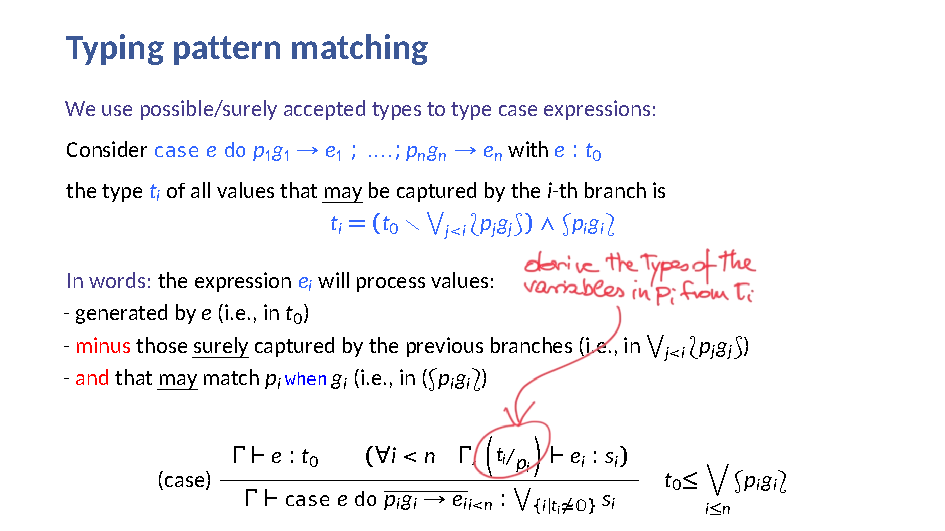
\includegraphics[scale=1]{images/slide-caserule1.pdf}
\end{textblock}}
\only<9>{\begin{textblock}{5}(0,0)
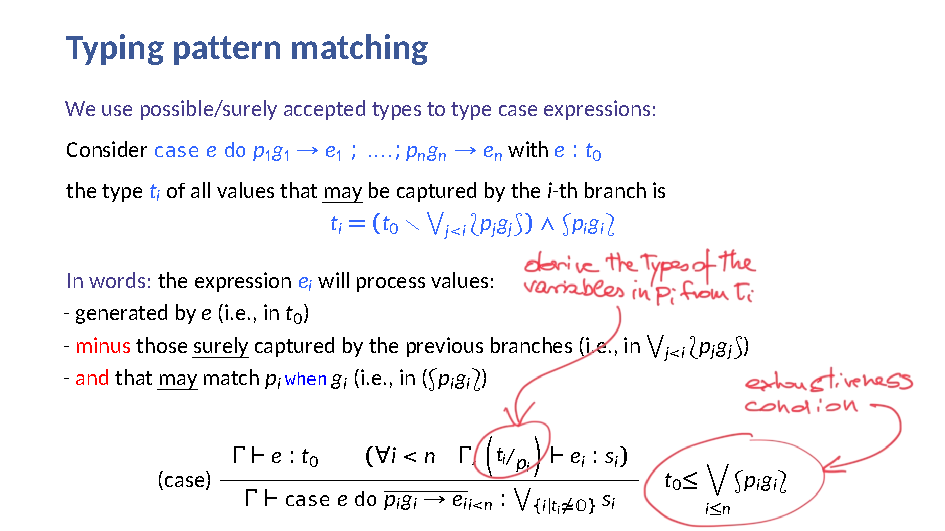
\includegraphics[scale=1]{images/slide-caserule2.pdf}
\end{textblock}}
\only<10>{\begin{textblock}{5}(0,0)
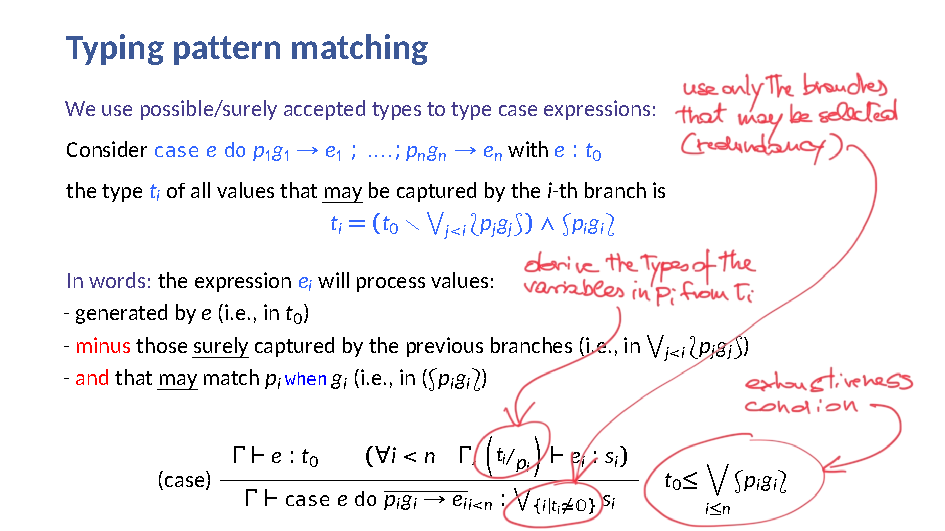
\includegraphics[scale=1]{images/slide-caserule3.pdf}
\end{textblock}}
\end{frame}



\begin{frame}[fragile]
\frametitle{Precise Guard Analysis}

\textbf{\color{darkslateblue}For each pattern guard we deduce a \emph{list} of flagged types (by decomposing the guard in OR-clauses):}
\vspace{-2mm}
\[\Gamma\vdash p_ig_i \leadsto [(s_{ij},\BoolB_{ij})]_{j\leq m_i}\]


%\only<2>{\vspace{-1.7mm}}

\

% \pause\pause
% \only<3>{\begin{textblock}{5}(0,0)
% \includegraphics[scale=1]{images/guardanalysis1.pdf}
% \end{textblock}}
% \only<4>{\begin{textblock}{5}(0,0)
% \includegraphics[scale=1]{images/guardanalysis2.pdf}
% \end{textblock}}

\pause\pause
\pause 
\begin{block}{Guard Analysis}
Consider again \quad $pg$ \quad =\quad   {\color{typeGreen}\code{x when (is_map(x) and map_size(x) == 2) or
  is_list(x)}}
\pause
   $\Gamma,\texttt{term()}\vdash [ pg ] \leadsto$ [(\code{map()},\code{false}),
      (\code{list()},\code{true})]

\pause
    $\sAccType{pg}\quad=\quad$  {\color{typeGreen}\code{list()}}\hfill (all types in the list with
\code{true} flag)\vspace{-1mm}

    $\pAccType{pg}\quad=\quad$   {\color{typeGreen}\code{map() or list()}} \hfill (all types in the
list with any flag)

\end{block}
\pause
\structure{\bf Fine-grained analysis needed to  infer the type of}
\begin{minted}{elixir}
def baz(x, y) when is_boolean(x) or is_integer(y), do: {y,x} 
#=> ((term(),integer()) -> {integer(),term()}) and
#   ((boolean(),term()) -> {term(),boolean()})
\end{minted}
\only<2>{\begin{textblock}{5}(0,0)
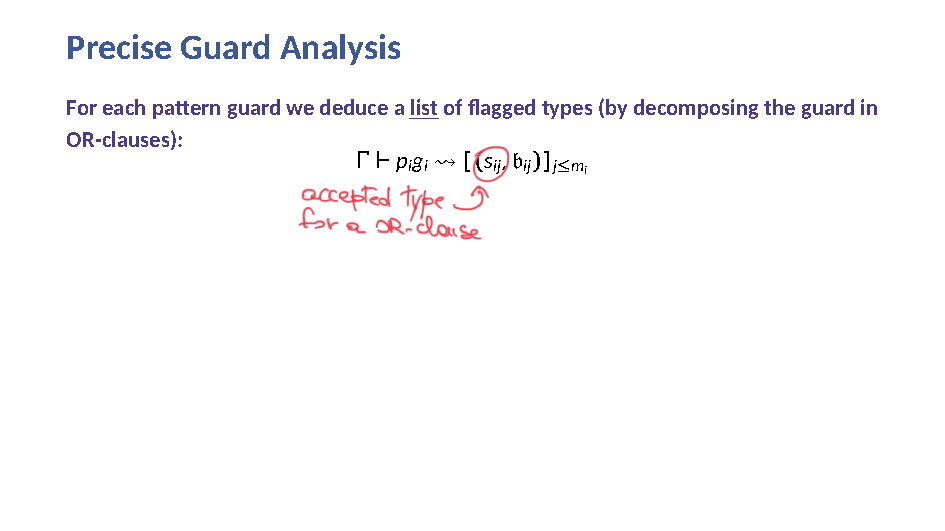
\includegraphics[scale=1]{images/slide-guardtype.pdf}
\end{textblock}}
\only<3>{\begin{textblock}{5}(0,0)
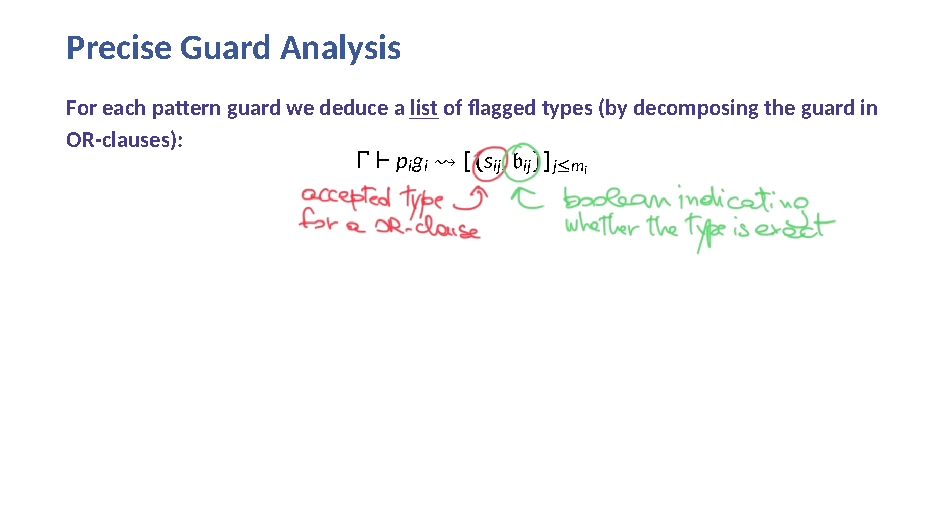
\includegraphics[scale=1]{images/slide-guardbool.pdf}
\end{textblock}}
\end{frame}


\section{Gradual Typing}

\begin{frame}
\frametitle{Outline} 
\tableofcontents[currentsection]
\end{frame}

\begin{frame}
\frametitle{Gradual typing}\transdissolve<2>
\begin{block}{Principles}
\begin{itemize}
\setlength{\itemsep}{-2pt}
\item Blend statically typed and dynamically typed code
\item Gradual migration instead of converting entire codebase at once
\item Introduce \code{dynamic()} type for type-checking in dynamic typing mode
\end{itemize}
\end{block}

\begin{block}{The \code{dynamic()} type}
\begin{itemize}
\setlength{\itemsep}{-0pt}
\item May turn into any other type at runtime
\item Offers a more relaxed type safety guarantee:\\
 \color<2>{purple}If some program \code{e} has type \code{integer()} and evaluates to a value, \\
      then this value is of type \code{integer()}.
\end{itemize}
\end{block}
\pause\vspace{-4mm}
\begin{exampleblock}{\vspace{-5mm}}
\centering\bf  Same guarantees as \emph{sound gradual typing} but {\color{purple}without inserting
  casts at compilation}
\end{exampleblock}

\end{frame}
%%% def boolean_id(x), do: x
\defverbatim[colored]{\weakApp}{
\begin{minted}{elixir}
id_weak(x_dyn)
# type dynamic()
\end{minted}
}
\defverbatim[colored]{\strongApp}{
\begin{minted}{elixir}
id_weak(x_dyn)                    id_strong(x_dyn)
# type dynamic()                  # type integer() 
\end{minted}
}
\defverbatim[colored]{\strongAppPropagation}{
\begin{minted}{elixir}
id_weak(x_dyn)                    id_strong(x_dyn)
# type dynamic()                  # type integer() !\color{magenta}and dynamic()!
\end{minted}
}

\begin{frame}
\frametitle{Gradual Typing Conundrum}
\textbf{\color{darkslateblue}Typing every expression by \code{dynamic()} is trivially sound \ldots but hardly useful.}

\bigskip
\pause
The system must fulfill two opposite requirements
\begin{enumerate}
	\item it must use \code{dynamic()}  as little as possible so as to be useful, and
	\item it must use \code{dynamic()} enough so as not to hinder the versatility of
	      gradual typing
\end{enumerate}


\bigskip
\pause
The first requirement is fulfilled by the typing of \textbf{\color{darkslateblue}strong functions}, which leverage the run-time checks written by the programmer, or performed by the VM\\[3mm]
The second requirement is fulfilled by the \textbf{\color{darkslateblue}propagation of \code{dynamic()}}.
\end{frame}

\subsection{Strong function types}

\begin{frame}[fragile]{Strong function types}\transdissolve<2,4->
\vspace{-1.5mm}
\begin{block}{(Weak) function type}
\begin{minted}[escapeinside=!!]{elixir}
!\spec! integer() -> integer()
def id_weak(x), do: x !\label{c1}!
\end{minted}
\end{block}
\vspace{-1.6mm}
\pause
\begin{block}{Let \code{x_dyn} be of type \code{dynamic()}}
\vspace{-4.9mm}
    \begin{overlayarea}{\textwidth}{1.3cm}
        \only<2-3>{\weakApp}
        \only<4-7>{\strongApp}
        \only<8>{\strongAppPropagation}
   \end{overlayarea}
\end{block}
\vspace{-1.5mm}
\pause
\begin{block}{Strong function type \only<6->{\smash{(by the programmer)}}}
\begin{minted}[linenos=false,escapeinside=!!]{elixir}
!\spec! integer() -> integer()
def id_strong(x) when is_integer(x), do: x 
\end{minted}
\end{block}
% \begin{block}{Application}
% \begin{minted}{elixir}
% !\spec! dynamic() -> {dynamic(), integer()}
% def dynamic_fun(x), do: {id_weak(x), id_strong(x)}
% \end{minted}
% \end{block}
\pause\pause\pause\pause
\vspace{-.5mm}
% \frametitle{Strong function types (by the VM)}
\begin{block}{Strong function type (by the VM)}
\begin{minted}[linenos=false,escapeinside=!!]{elixir}
!\spec! integer() -> integer()
def double(x), do: x + x
\end{minted}
\end{block}
% \begin{itemize}
% \item Functions with strong types guarantee correct output or runtime type-check failure
% \item Ensures stronger type safety guarantee without modifying Elixir compilation
% % \item Take into account user type checks
% % \item Allows for propagation of \code{dynamic()} type in certain cases
% \end{itemize}
\only<5,6>{\begin{textblock}{15}(1.3,13.5)
    \textbf{\color{darkslateblue}\large Strong function types guarantee correct output or runtime type-check failure}
\end{textblock}}
\only<9>{\begin{textblock}{5}(0,0)
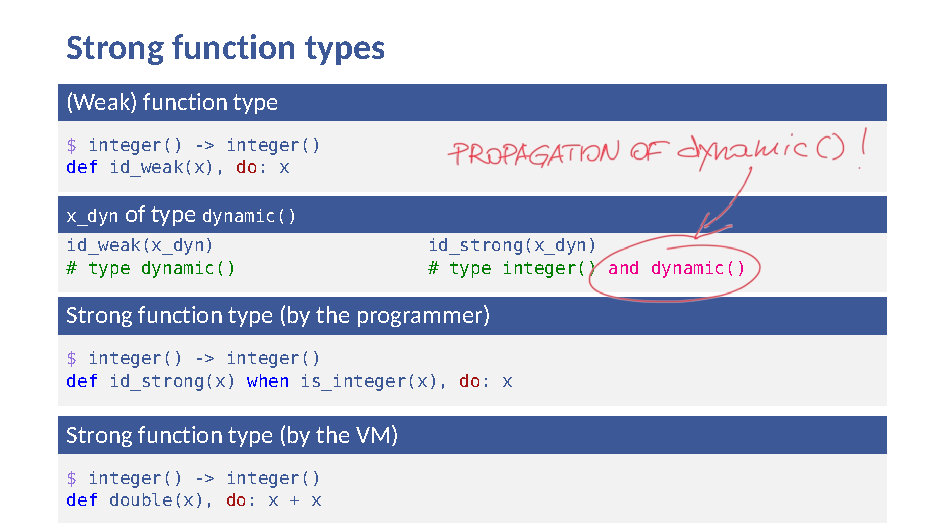
\includegraphics[scale=1]{images/slide-dynprop.pdf}
\end{textblock}}
\end{frame}




\defverbatim[colored]{\dynType}{
\begin{minted}{elixir}
#=> Result type: (integer() or boolean()) !\color{magenta}and dynamic()!
\end{minted}
}
\defverbatim[colored]{\wrongType}{
\begin{minted}{elixir}
#=> Possible type: integer() or boolean()
\end{minted}
}
\defverbatim[colored]{\typeError}{
\begin{minted}{elixir}
#=> Type Error: + undefined for booleans
\end{minted}
}
\defverbatim[colored]{\goodType}{
\begin{minted}{elixir}
#=> Result type: integer()
\end{minted}
}
\defverbatim[colored]{\betterType}{
\begin{minted}{elixir}
#=> Result type: integer() and dynamic()
\end{minted}
}
\defverbatim[colored]{\subtract}{
\begin{minted}{elixir}
def subtract(a, b) do
    a + negate(b)
\end{minted}
}
\defverbatim[colored]{\subtractann}{
\begin{minted}{elixir}
def subtract(a, b) do               !\textcolor{gray}{\footnotesize//if b is given an argument of type dynamic()}!
    a + negate(b)
\end{minted}
}

\subsection{Propagation of \texttt{dynamic()}}

\begin{frame}[fragile]{Propagation of \texttt{dynamic()}}\transdissolve<6>
\textbf{\color{darkslateblue}Apply the (strong function) \code{negate()} function to a \code{dynamic()} argument:}
\vspace{-4mm}
\begin{block}{\vspace{-5mm}}
\begin{minted}{elixir}
!\spec! (integer() -> integer()) and (boolean() -> boolean())
def negate(x) when is_integer(x), do: -x
def negate(x) when is_boolean(x), do: not x
\end{minted}
\vspace{-6.1mm}
\begin{overlayarea}{\textwidth}{2mm}
    \only<2-5>{\wrongType}
    \only<6->{\dynType}
\end{overlayarea}
\hfill
\vspace{1.7mm}
\hfill
\end{block}
\pause\pause\vspace{-6mm}
\begin{block}{\vspace{-6mm}}\vspace{-2mm}
\begin{overlayarea}{\textwidth}{13mm}
\only<3,6>{\subtract}
\only<4,5,7->{\subtractann}
\end{overlayarea}
\vspace{-6.5mm}
\begin{overlayarea}{\textwidth}{2mm}
    \only<5>{\typeError}
    \only<8>{\goodType}
    \only<9->{\betterType}
\end{overlayarea}
\hfill
\vspace{1.7mm}
\end{block}
\pause\pause\pause\pause\pause\pause\pause\vspace{-6mm}
\begin{block}{\vspace{-5mm}}
\begin{minted}{elixir}
def concat(a, b) do
    a ++ negate(b) 
end
#=> Type Error: incompatible types.
\end{minted}
\end{block}
\end{frame}



\section{Integration in Elixir}

\begin{frame}
\frametitle{Outline} 
\tableofcontents[currentsection]
\end{frame}

\begin{frame}
\frametitle{Status of the Integration}\vspace{-4mm}
\begin{itemize}\setlength{\itemsep}{1pt}
\item Integration started in version 1.17 of Elixir, with type structures and gradual typing
\item version 1.18 covered more types and type-checked function calls performing type
inference for patterns and return types by refined guard analysis  
\item The current v1.19 
covers all language constructs and includes basic, atom, tuple, list, map, and
function types, as well as the typing of \textit{protocols} (akin to type classes in Haskell). The forthcoming 1.20 (rc4) covers all the inference for functions. \textcolor{darkslateblue}{No type annotations and no parametric polymorphism, yet}.
\end{itemize}
\pause\smallskip

\small
\begin{tabular}{|l|r|r|r|r|r|r|}
\hline\rowcolor{violet2}
Codebase & \multicolumn{1}{c|}{LoC} & \multicolumn{1}{c|}{Files} & Modules & \makecell{Type Checking\\ Time} & \makecell{Total Compilation\\ Time} & \multicolumn{1}{c|}{\%}\\[-1pt]
\hline
Remote & $>$1,000,000 & $>$10,000 & 18,059 & 11.116 s & 707.598 s  & 1.6\\[-1.5pt]
\rowcolor{violet1}
Livebook & 61093 & 254 & 299 & 0.177 s & 4.112 s&4.3\\[-1.5pt]
Credo & 29181 & 252 & 264 & 0.059 s & 1.305 s &4.5\\[-1.5pt]
\rowcolor{violet1}
Phoenix &  21389& 71& 88 &  0.049 s& 0.525 s&9.3\\[-1.5pt]
Hex & 15632 & 196 & 241 & 0.091 s & 1.339 s  &6.8\\[-1pt]

\hline
\end{tabular}\pause

\bigskip
\textbf{\textcolor{darkslateblue}{\large Discovered type errors in all of them}}   
\end{frame}


\begin{frame}[fragile]
\frametitle{Status of the Integration}\vspace{-3mm}
\begin{itemize}
\item Very positive feedback from developers on versions 1.17 and 1.18
\item No syntactic changes required to Elixir code was particularly appreciated
\item Uncovered previously hidden errors without significant overhead
\item Found issues in major projects: Phoenix, Livebook, Postgrex, and Flame that persisted undetected in production, sometimes for years
\end{itemize}

\bigskip\pause

\begin{block}{Real-world Bug Discoveries}
\begin{itemize}
    \setlength{\itemsep}{0pt}
\item \textbf{Phoenix}: Critical type mismatch in \code{String.to_atom/1} \hfill\small (deployed on 12,000+ websites)
\item \textbf{Postgrex}: 15 lines of dead code removed
\item \textbf{Flame}: 2 dead code paths found via guard analysis
\item \textbf{Live-view}: 6 lines of dead code removed
\item \textbf{Remote}: detected a critical type mismatch application\\ undetected by tests because in an error branch that is rarely executed.\vspace{-1mm}
\end{itemize}
\end{block}
\end{frame}

\begin{frame}[fragile]
\frametitle{\mbox{Other Languages using (more or less) Semantic Subtyping:}}
\begin{itemize}\setlength{\itemsep}{0pt}
    \item CDuce (and currently its spin offs: SSTT and MLsem)
    \item Ballerina (by WSO2) uses semantic subtyping since its Swan Lake release
    \item Luau (by Roblox)uses semantics subtyping when its syntactic subtyping fails.
    \item R (Jan Vitek's group has being developing a type system for R based on semantic subtyping)
    \item Julia developers affirm to have drawn inspiration from Semantic Subtyping for the type system.
    \item Python (\textsf{ty}, the high-performance Python type checker developed by astral, uses semantic subtyping and several low-level data-structures and optimizations developed for Elixir to implement semantic types) 
    \item Ethylizer (uses semantic subtyping type reconstruction to type-check unannotated Erlang code)
    \item eqWAlizer (use semantic subtyping to type WhatsApp Erlang code)
\end{itemize}
\end{frame}

\begin{frame}[fragile]
\frametitle{Future work}\vspace{-2mm}[In order of state of completion]

\bigskip
\textbf{\color{darkslateblue}Types for the Elixir Module System:}\\
Currently, only the type \code{module()} is supported, while we want a finer-grained typing of functions manipulating modules:\vspace{-5mm}
\begin{block}{\vspace{-25mm}}
\begin{minted}{elixir}
!\spec! (X: Stack[el=bool], sx: X.stack, Y: Stack[el=bool], sy: Y.stack) -> Y.stack
def move(X, sx, Y, sy), do: Y.push(sy, X.top(sx))   
\end{minted}
\end{block}

\bigskip
\textbf{\color{darkslateblue}Record types comprehensions:}\\
We want to type standard library functions that manipulate records with \emph{first-class} keys, such as \code{Map.intersect/2} and \code{Map.reject/2}.
\definecolor{typeconstructorgreen}{rgb}{0.0, 0.5, 0.25}  % Nice green for type constructors
\definecolor{keyvarblue}{rgb}{0.1, 0.3, 0.7}              % Nice blue for key variables
\newcommand{\keyof}[1]{\textcolor{typeconstructorgreen}{\mathsf{keyof}}(#1)}
\newcommand{\tvar}{\textcolor{keyvarblue}{\boldsymbol{\theta}}}
\begin{tabular}{@{}l@{\;\;}l@{\;\;}l@{}}
 \texttt{intersect/2}
  & $(\alpha,\, \beta) \to \%\{\,\tvar \in \keyof{\alpha} \land \keyof{\beta} \mid \beta[\tvar]\,\}\quad\texttt{when } \alpha,\beta\texttt{:map()}$  \\[6pt]
\texttt{reject/2}
  & $(\alpha, ((\keyof{\alpha} \to \texttt{term}) \,\wedge\, ( \keyof{\alpha}\wedge\beta)\to\neg\texttt{truthy})) \to $\\
  &\qquad\qquad\qquad\qquad
     $\%\{\, \tvar\in \keyof{\alpha}\setminus\beta \mid \alpha[\tvar]\,\} \quad\texttt{when } \alpha\texttt{:map()}$\\[3pt]
\end{tabular}
\end{frame}
\begin{frame}
\bigskip
\textbf{\color{darkslateblue}Types for processes and message passing:}
Currently, only the type \code{pid()} is supported.

We are working on typing processes with the set of messages they can receive and later, introduce Mailbox types, to ensure liveness properties.


\bigskip
\textbf{\color{darkslateblue}Tooling:} We are developing migration tools, IDEs, error messages, .... In particular, we are  feeding LLMs with automatic translations of Typespecs into Elixir Types together with the type errors they produce to improve the quality of LLM-generated type annotations and error messages.


\bigskip
\textbf{\color{darkslateblue}Implementation:}
\begin{itemize}\setlength{\itemsep}{-2pt}
\item v1.20 completion of inference for functions
\item v1.21 first modification of the language: explicit type annotation for structs
\item v1.22 \code{!\color{darkgreen}\$!}-prefixed  type annotations for functions
\item later: polymorphic types, row polymorphism, polymorphic inference, ...
\end{itemize}
\end{frame}



\begin{frame}[fragile]
\frametitle{References}


\textbf{\color{darkslateblue}On Elixir Typing:}
\begin{itemize}\setlength{\itemsep}{2pt}
    \item[[\,1\!\!]] G. Castagna, G. Duboc, and J. Valim: \textit{The Design Principles of the Elixir Type System}. The Art, Science, and Engineering of Programming, vol.8, n.2, 2024.
    \item[[\,2\!\!]] G. Castagna and G. Duboc: \textit{Guard Analysis and Safe Erasure Gradual Typing: a Type System for Elixir}, 7, 2025. Submitted for publication (available on my web page).
\end{itemize}


\textbf{\color{darkslateblue}On Set-Theoretic types:}
\begin{itemize}\setlength{\itemsep}{2pt}
    \item[[\,3\!\!]] G. Castagna: \textit{Programming with Union, Intersection, and Negation Types}. In \textit{The French School of Programming}, Springer, pag. 309―378, March, 2024. ISBN 978-3-031-34517-3. Preprint at \href{https://arxiv.org/abs/2111.03354}{arXiv:2111.03354}.
\end{itemize}
\end{frame}

\end{document}
